\documentclass[conference]{IEEEtran}
\IEEEoverridecommandlockouts
% The preceding line is only needed to identify funding in the first footnote. If that is unneeded, please comment it out.
\usepackage{cite}
\usepackage{amsmath,amssymb,amsfonts}
\usepackage{algorithmic}
\usepackage{graphicx}
\usepackage{textcomp}
\usepackage{xcolor}

%%librerías añadidas
\usepackage{fancyhdr}
\usepackage{graphicx}
\usepackage[spanish, es-tabla]{babel}
\usepackage[utf8]{inputenc}
\usepackage{color}
\usepackage{hyperref}
\usepackage{wrapfig}
\usepackage{array}
\usepackage{multirow}
\usepackage{adjustbox}
\usepackage{nccmath}
%\usepackage{anysize}
\usepackage{subfigure}
\usepackage{amsfonts,latexsym} 
\usepackage{enumerate}
\usepackage{booktabs}
\usepackage{float}
\usepackage{threeparttable}
\usepackage{array,colortbl}
\usepackage{ifpdf}
\usepackage{rotating}
\usepackage{cite}
\usepackage{stfloats}
\usepackage{url}
\usepackage{listings}

\usepackage{verbatim} % comentarios
%%%%%%%%%%%%%%%%%%%
\def\BibTeX{{\rm B\kern-.05em{\sc i\kern-.025em b}\kern-.08em
    T\kern-.1667em\lower.7ex\hbox{E}\kern-.125emX}}
\begin{document}

\title{Implementación dispositivo CNC \\a partir de GRBL}

\author{\IEEEauthorblockN{1\textsuperscript{st} Juan  Masmela }
\IEEEauthorblockA{\textit{dept. Electronic engineering} \\
\textit{Universidad Central}\\
Bogotá, Colombia \\}

}

\maketitle

\begin{abstract}
En este documento se ve redactado el desarrollo e implementación de un dispositivo CNC a partir de el software GRBL,  dando un contexto histórico y ilustrativo, describiendo su construcción  física, los materiales que se usaran para su implementación  y codificación del software con el fin de fabricar placas de circuito base PCB con facilidad. 

\end{abstract}

\begin{IEEEkeywords}
CNC, GRBL, PCB  .
\end{IEEEkeywords}

\section{Introducción}
Un inconveniente al momento de diseñar una solución electrónica es la elaboración de un circuito, las dificultades que presenta a momento de hoy son los tiempos de envió de las placas de China y como en caso de cometer un error de diseño los tiempos de envió generan mas perdida que beneficio.\\
para solventar esos inconvenientes los desarrolladores de hardware a menor escala procuran tener el mejor diseño, pero los errores son frecuentes, una solución a estos inconvenientes parte de reducir los tiempos de desarrollo interviniendo directamente en los tiempos de envíos de las PCB, esto se logra facilitando el desarrollo de las mismas a partir de que los desarrolladores las elaboren partiendo de dispositivos estrictamente diseñados para este proceso.\\
Uno de los dispositivos frecuentemente usado para la elaboración de PCB son las maquinas CNC (control numérico computarizado), estos dispositivos a partir de instrucciones establecidas son capaces de hacer una abarcón a las placas de baquelita cubiertas de cobre, para dar forma a las mismas.\\
Estas maquinas a fecha de este documento son ampliamente elaboradas por su versatilidad y practicidad por todo tipo de entusiastas que desean poseer una, gracias a esto hay proyectos de código abierto que permiten a cualquier persona con los recursos necesarios implementar proyectos donde son requeridas.\\
\\A efectos de este documento se describirá como se desarrolla una maquina cnc con el fin de elaborar PCB partiendo de los archivos generados por los software de diseño de circuitos, para ello se tomaran software de código abierto y partiendo de los diseños propuestos en estos se elaborara la maquina CNC con los requerimientos propuestos; En este documento se encuentra una referencia del desarrollo de estos dispositivos, sus componentes, como se desarrollara el mismo, como se elaborara el montaje físico del dispositivo, en que se caracteriza, pruebas experimentales y conclusiones del proyecto. 


\section{Marco teórico}
\subsection{breve contexto histórico}
En la búsqueda de datos, la implementación de maquinas de control numérico computarizado se data desde la década de los 80s, estos siendo modelos de control de lazo cerrado \cite{b0}, y tipos de control óptimos para maquinaria controlada \cite{b1}; Destacando que en el desarrolló de estos dispositivos se buscaba la forma mas óptima de generar el orden de instrucciones para las maquinarias, ya sea destacando su estructura, área, método de implementación de instrucciones y sistemas de control para cada requerimiento que se desarrollase.\\ 
Años posteriores, por la década de los 2000, con el auge de microcontroladores económicos y de mejores capacidades, se busco implementar de forma mas económica estos dispositivos ya sea para el desarrollo de maquinas CNC o dispositivos de impresión en $3 D$. La implementación de estas maquinas en entornos industriales conlleva un gran costo, donde en algunos casos se implementaban proyectos de software libre \cite{b6}; ya para proyectos posteriores al año 2010 la aparición de módulos diseñados con el fin de controlar motores paso a paso aparecieron por el mercado, donde el estudio estructural de los diseños de las maquinas empiezan a aparecer \cite{b10}  y mas a futuro con los intentos de implementación reglamentada y verificación de los margenes de error de las propias maquinas que implementan su propio software a partir del uso de PLC \cite{b2}, y no solo del uso de hardware de alto valor, también implementaciones con material reciclado \cite{b5}, y la proliferación de softwares libres para montajes de menor escala con un nivel de complejidad mas moderado \cite{b11}.\\ Con la aparición de dispositivos específicamente diseñados para el frezado de madera y la implementación de PCB de forma rápida para la creación de piezas mecánicas de difícil desarrollo a mano \cite{b7}; Para instantes de tiempo mas contemporáneos a la redacción de este documento el uso de softwares  especializados con un hardware especifico como el GRBL ya sea para 2 o 3 ejes \cite{b13}, y la aplicación del mismo pero con materiales reciclados a una menor escala y menor costo para dibujar \cite{b12}. Para aplicaciones especializadas el diseño y creación de piezas especificas en materiales metálicos y que sea fácil de adecuar para procesos industriales  \cite{b4}.
Una característica de las implementaciones anteriormente vistas es el uso de controladores de pasos para los motores como lo son el driver $"L293D"$ , $"L298n"$, $"A4988"$, $"Tmc2209"$, y $"DRV8825"$ \cite{b8}. Ya con mejores criterios de diseño físico para implementaciones industriales de baja y media escala usando como base el software GRBL \cite{b9}.Otra característica determinante es el uso del software universal Gcode sender, el cual traduce las instrucciones para la interpretación del dispositivo y su respectivo funcionamiento automático \cite{b3}.\\

Con todo lo mencionado anteriormente se denota la necesidad de poder crear todo tipo de piezas de forma automática desde que se formalizo la necesidad, esto a conllevado a un desarrollo fácil de implementar y en lo posible que sea económico como criterios determinantes. 





\subsection{microcontrolador y módulos anexos}
para el microcontrolador se uso un Atmega328p \cite{micro} embebido en una placa arduino uno \cite{arduino} de la que se destaca su versatilidad al momento de implementar cualquier proyecto, anexo a este va un driver cnc shield \cite{shield} el cual esta diseñado para acoplar los drivers de los motores que contienen el integrado DRV8825 \cite{pololu}.


% 

\section{Solución propuesta}
La solución a desarrollar es una CNC para elaboración de PCB, teniendo en cuenta que La precisión es un factor determinante; Ya con los criterios principales planteados se deven delimitar los criterios fisicos como el area de frezado, el material y la precisión .\\ 
Un factor a destacar de la solución propuesta es el uso del software GRBL \cite{b13} \cite{GRBL}, este es un desarrollo de código abierto que caracteriza los movimientos que presentara la maquina a partir de la codificación de instrucciones Gcode que se generaran a partir de un programa que procesara los archivos generados por los software de diseño de pcb y modelado en $3 D$ a instrucciones procesables.\\ 
Una característica determinante es la implementación física, esta se elaboro a partir de un chasis también de uso libre, el cual es el mas recomendado en conjunto con GRBL, aunque en función del área donde se pretende trabajar en el propio código hay constantes que se pueden variar en función del criterio de ensamblaje.


\section{Desarrollo del Dispositivo}
Para la implementación física del dispositivo se parte contar con los materiales estrictamente necesarios para el ensamblaje, esto teniendo en cuenta los planos del uso de 3 ejes que se componen de varas de soporte y un eje de barras dentadas, el cual dará los movimientos a partir de motores paso a paso; El soporte estructural es de madera con la forma característica necesaria para la estructura. 

 \begin{figure}[htb]
        \centering
        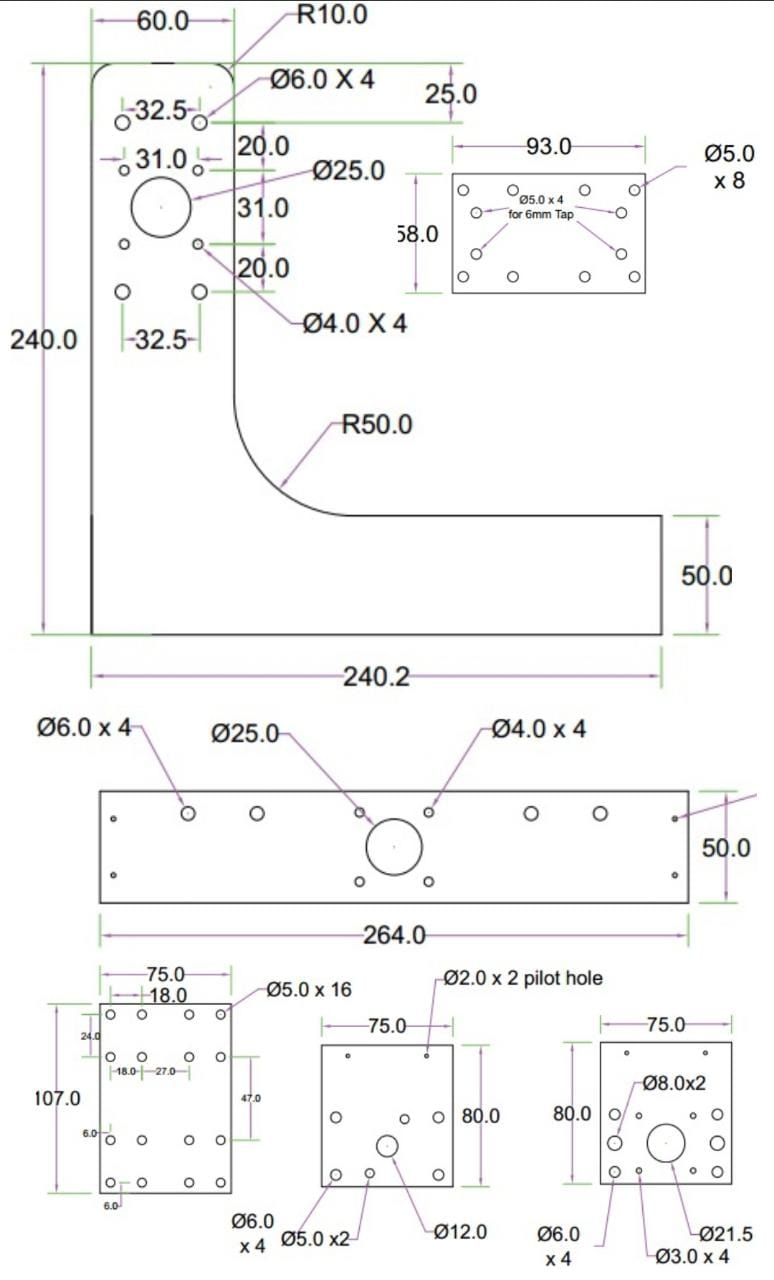
\includegraphics[width=0.28\textwidth]{planos.PNG}
        \caption{Planos estructura de la CNC }
        \sucaption{\textit
        {En esta imagen se pueden ver los planos de la estructura física de la CNC }
        \label{fig:Planos-cnc}}
        \end{figure}

Ya con los planos propuestos \ref{fig:Planos-cnc} el siguiente paso es ilustrar como funciona el sistema eléctrico de la CNC, para ello se debe tener en cuenta que esta posee 3 motores nema 17, los módulos DRV8825, la CNC shield y la placa Arduino todo alimentado con la misma fuente de alimentación.\\


 \begin{figure}[htb]
        \centering
        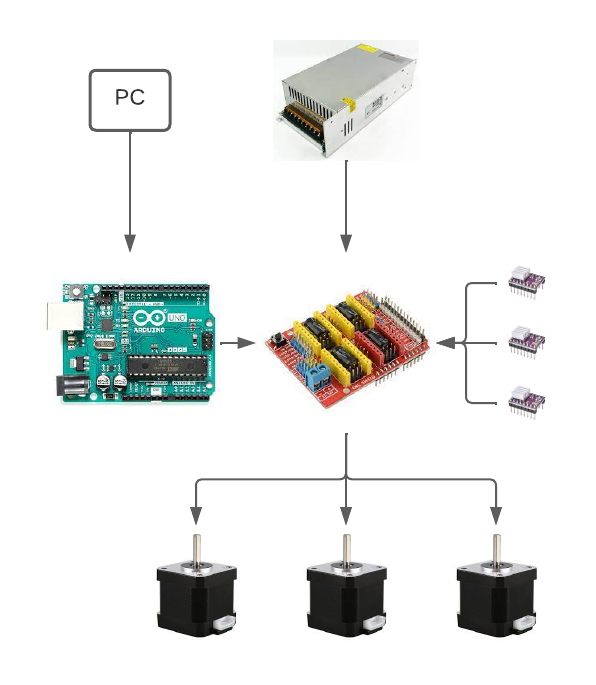
\includegraphics[width=0.31\textwidth]{bloques cnc.png}
        \caption{Diagrama de bloques de componentes eléctricos de la CNC }
        \sucaption{\textit
        {En esta imagen se puede ver el montaje eléctrico en bloques de la CNC }
        \label{fig:electrico-cnc}}
        \end{figure}
  
  Un detalle a destacar es la calibración de los módulos DRV8825, para esto en las especificaciones de pololu del driver indican lo siguiente\cite{ti_DRV8825}:
  \begin{equation}
      V_{ref}=I_{Max}(5(R_s))
  \end{equation}
  Donde $I_{Max}$ corresponde a la corriente de funcionamiento de los motores nema 17, para este caso son $1.7A$; Otro factor a destacar es $R_s$, este viene dado por el modulo controlador de pololu \cite{pololu}, donde al observar el modulo la resistencia es de $0.1\Omega$, denotando la siguiente ecuación:
  
  \begin{equation}
      1.7_{A}(5(0.1\Omega)) =850_{mv}
  \end{equation}
  
  
 
  No obstante para un mejor rendimiento a largo plazo se trabaja al $70\%$ dado que se trabaja a pasos completos dando como resultado ${\color{Red} 595_{mv} }$ de tensión de control máxima.\\
Teniendo los valores anteriormente mencionados como referencia los driver se regulan a la tensión mínima en los que los motores empiezan a girar, esto varia según la obstrucción mecánica del propio chasis.\\
\\
Para la calibración de los pasos es necesario identificar cuantos pasos por grado da el motor, para ello al observar la hoja de especificaciones de los motores nema 17 se destaca que los pasos son de $1.8$ por grado, para identificar los pasos se hace lo siguiente:
 \begin{equation}
      \frac{360}{1.8}=200
  \end{equation}
  
  Ya con los pasos identificados lo siguiente es identificar como funcionan los ejes, estos avanzan $4mm$ por vuelta para lo cual se identifica que:
  
   \begin{equation}
      \frac{200}{4}=50
  \end{equation}
  
  Este valor corresponde a una constante de calibración que se ingresa en la memoria del microcontrolador; Aunque para una mejor precisión, lo óptimo es identificar cuanta distancia recorre en cada uno de los ejes  y a partir de esto se calculan los nuevos pasos que debe dar por eje, donde\\
  
     \begin{equation}
      \frac{(dimensiónreq*pasospormm)}{dimensiónobtenida
} = pasos
  \end{equation}
  \\
  
 \\Un factor a destacar es que el motor de la frezadora puede funcionar de forma independiente, no obstante se pretende que la misma fuente de alimentación da energía al motor usando un modulo regulador de voltaje y posterior a este un regulador de velocidad para el motor; Considerando el inconveniente de los costes de estos componentes, para efectos de calibración y demostración de funcionamiento se acoplara un bolígrafo el cual denotara los resultados en cualquier superficie que se especifique. \\ 

Ya con lo visto anteriormente se procede a hacer el montaje físico, integrando el montaje físico con el hardware.\\

 \begin{figure}[htb]
        \centering
        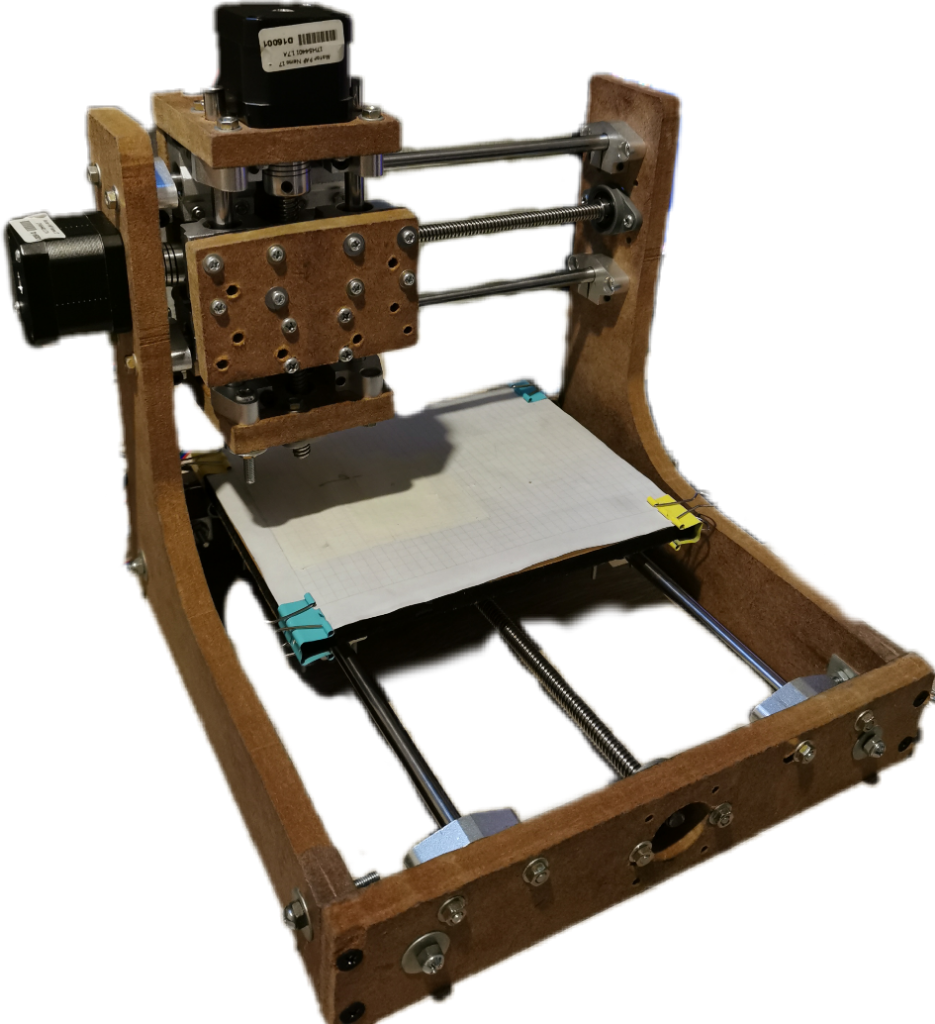
\includegraphics[width=0.3\textwidth]{CNC_.png}
        \caption{Implementación física chasis CNC }
        \sucaption{\textit
        {En esta imagen se puede ver el montaje físico estructural de la CNC }
        \label{fig:fisico-cnc}}
        \end{figure}


\\
\section{Pruebas experimentales}
Para las pruebas experimentales se destaca que se usara un lapicero para rayar una superficie, esta superficie se compone de cinta de papel y una lamina de apoyo, donde se obtuvo lo siguiente:

 \begin{figure}[htb]
        \centering
        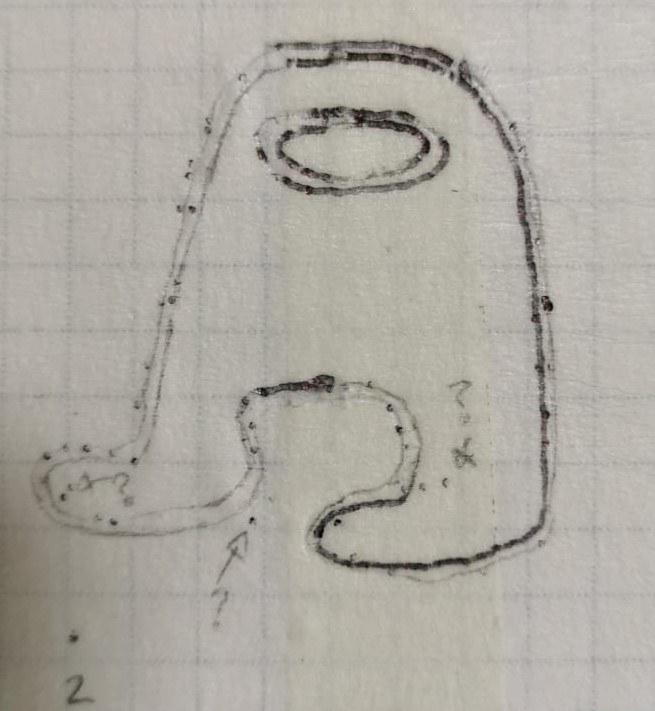
\includegraphics[width=0.3\textwidth]{sus.jpg}
        \caption{Prueba Superficial Básica CNC }
        \sucaption{\textit
        {En esta imagen se puede ver sus }
        \label{fig:sus}}
        \end{figure}
En la imagen \ref{fig:sus} podemos ver el resultado, destacando que la imagen se proceso tal cual es y se envió el resultado a la maquina, los espacios donde no rallo bien fue por la propia textura de la cinta y el tipo de lapicero a usar.\\

Para la siguiente prueba se cambiara tanto de lapicero como de superficie, esto se hace para identificar que independiente de la superficie los resultados son buenos, añadido a esto se hace un procesado de la imagen con el fin de generar una mejor vectorización que se ve reflejada en el resultado

 \begin{figure}[htb]
        \centering
        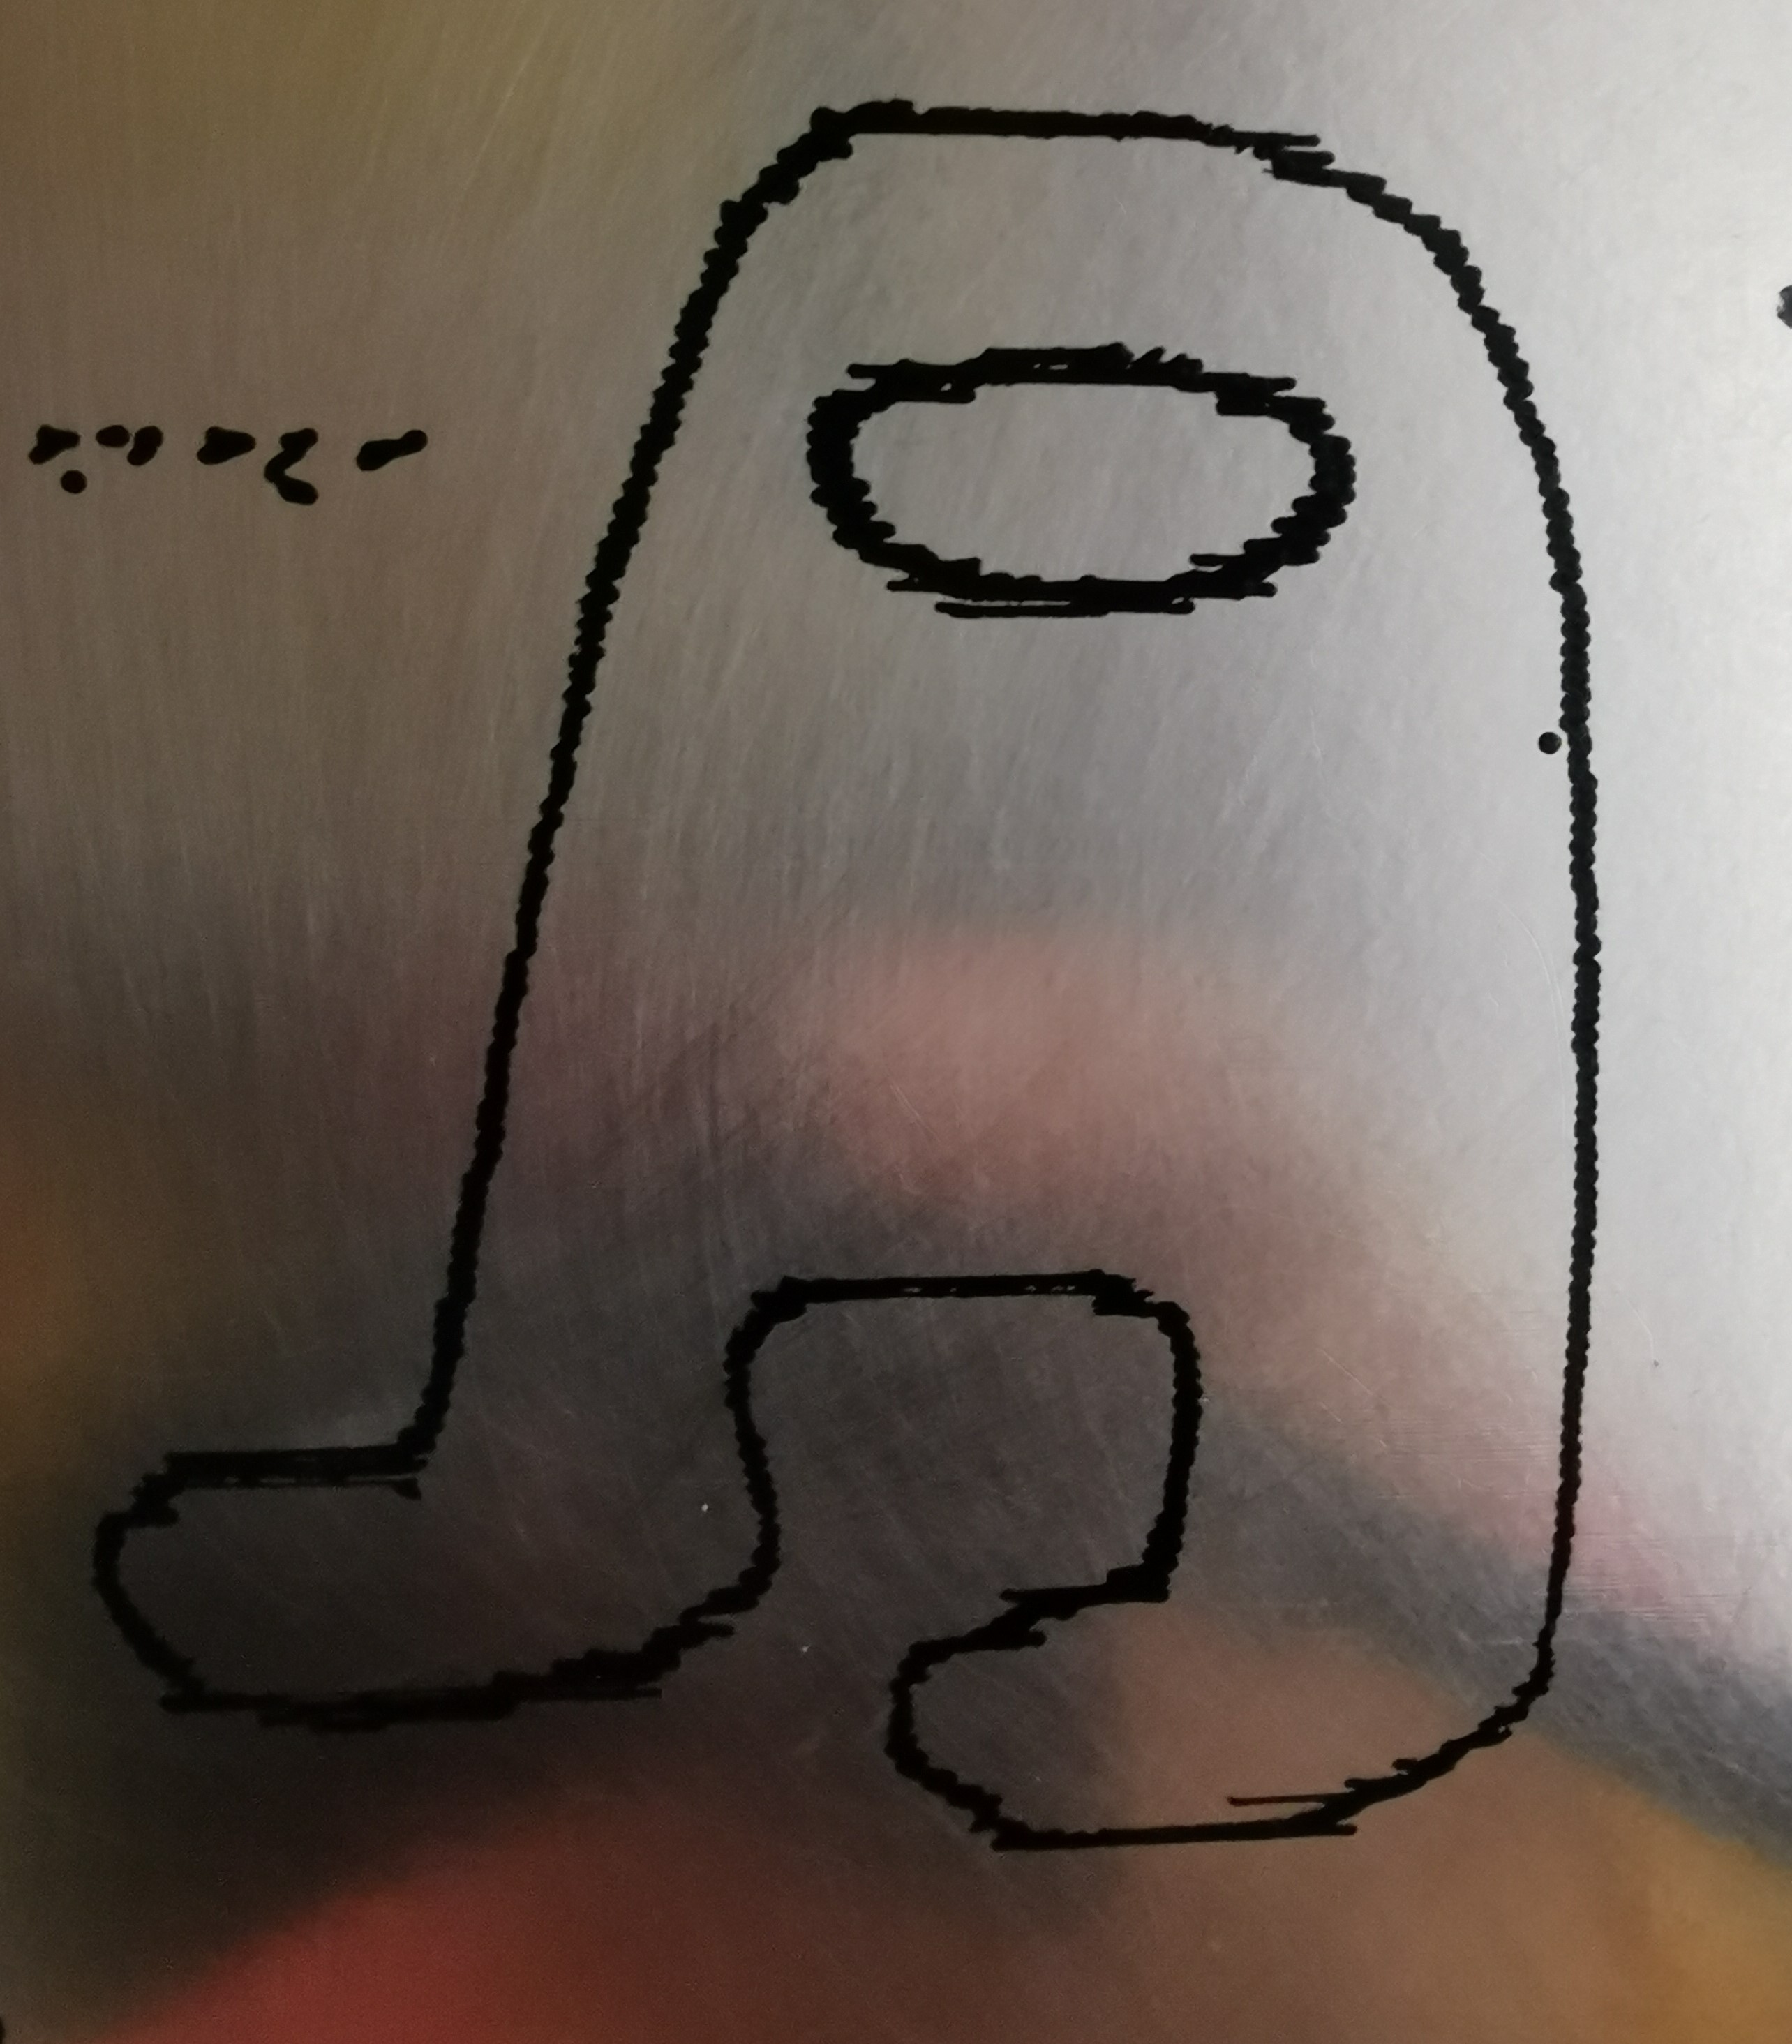
\includegraphics[width=0.3\textwidth]{SUS_COBRE.jpg}
        \caption{Prueba Superficial Básica CNC en placa de cobre }
        \sucaption{\textit
        {En esta imagen se puede ver sus }
        \label{fig:sus_cobre}}
        \end{figure}

\section{Conclusiones}
\begin{itemize}
    \item En la elaboración del proyecto se destaca que de base a fecha del documento la implementación es costosa, no obstante con una buena elaboración fomenta buenos resultados, denotando que el total de costes es $\$1156750$ pesos colombianos.

\end{itemize}
\begin{thebibliography}{00}
\bibitem{b0} Y. Koren and J. G. Bollinger, "Design Parameters for Sampled-Data Drives for CNC Machine Tools," in IEEE Transactions on Industry Applications, vol. IA-14, no. 3, pp. 255-264, May 1978, doi: 10.1109/TIA.1978.4503531.
\bibitem{b1} L. E. Schmitt, "PC Versus CNC-Which Do You Choose?," in IEEE Transactions on Industry Applications, vol. IA-20, no. 5, pp. 1141-1145, Sept. 1984, doi: 10.1109/TIA.1984.4504576.

\bibitem{b2} L. Chen, D. Yu, H. Zhang, C. Geng and L. Dong, "Design and implement of a modularized CNC interpreter based on the integration of tool path planning module," 2012 IEEE International Conference on Computer Science and Automation Engineering (CSAE), 2012, pp. 613-616, doi: 10.1109/CSAE.2012.6273027.

\bibitem{b3}N. Rastogi, H. Rastogi and N. Shrivastava, "Design and Implement an Economical Automatic CNC Wood Lathe Machine," 2021 4th International Conference on Recent Developments in Control, Automation & Power Engineering (RDCAPE), 2021, pp. 6-10, doi: 10.1109/RDCAPE52977.2021.9633378.

\bibitem{b4}V. Lawson, M. Phister and C. Rogers, " $A$utomated Rotor Assembly CNC Machine," 2020 Systems and Information Engineering Design Symposium (SIEDS), 2020, pp. 1-5, doi: 10.1109/SIEDS49339.2020.9106641.

\bibitem{b5}S. A. Membreno Vela, D. R. Martinez Garcia and J. J. Erazo Recinos, "Aplicación de tecnología moderna para la reutilización de lectores de CD/DVD: Implementation de CNC con materiales reciclados controlada con Arduino [Not available in English]," 2017 IEEE Central America and Panama Student Conference (CONESCAPAN), 2017, pp. 1-5, doi: 10.1109/CONESCAPAN.2017.8277611.


\bibitem{b6}Kittipong Ekkachai et al., "Design and development of an open architecture CNC controller for milling machine retrofitting," 2009 ICCAS-SICE, 2009, pp. 5629-5632.

\bibitem{b7}R. Choudhary, Sambhav, S. D. Titus, P. Akshaya, J. A. Mathew and N. Balaji, "CNC PCB milling and wood engraving machine," 2017 International Conference On Smart Technologies For Smart Nation (SmartTechCon), 2017, pp. 1301-1306, doi: 10.1109/SmartTechCon.2017.8358577.

\bibitem{b8}W. Wijaya, F. Syahroni, C. D. Mulyadi, W. Sani, A. Lukman and H. P. Nurba, "Two Axis Simple CNC Machines Based on Microcontroller and Motor Driver Shield IC L293D," 2020 14th International Conference on Telecommunication Systems, Services, and Applications (TSSA, 2020, pp. 1-5, doi: 10.1109/TSSA51342.2020.9310882.

\bibitem{b9}S. Shimabukuro, P. Díaz and L. Vinces, "Low cost semi-industrial 3GDL CNC vertical milling center design with non-ferrous metal machining capability," 2020 IEEE XXVII International Conference on Electronics, Electrical Engineering and Computing (INTERCON), 2020, pp. 1-4, doi: 10.1109/INTERCON50315.2020.9220260.

\bibitem{b10}Yu Yang, Wei Shengmin and Liu Ping," $A$ Universal Kinesiology modeling of multi-axis CNC machine," 2011 Second International Conference on Mechanic Automation and Control Engineering, 2011, pp. 45-48, doi: 10.1109/MACE.2011.5986853.

\bibitem{b11}W. A. Wibowo, T. Bagaswara and H. Nurhadi, "Prototyping a beneficial PC-based woodworking CNC machine WCM500 for creative industries," 2017 International Conference on Advanced Mechatronics, Intelligent Manufacture, and Industrial Automation (ICAMIMIA), 2017, pp. 300-305, doi: 10.1109/ICAMIMIA.2017.8387606.

\bibitem{b12}M. M. Hasan, M. R. Khan, A. T. Noman, H. Rashid, N. Ahmed and S. M. T. Reza, "Design and Implementation of a Microcontroller Based Low Cost Computer Numerical Control (CNC) Plotter using Motor Driver Controller," 2019 International Conference on Electrical, Computer and Communication Engineering (ECCE), 2019, pp. 1-5, doi: 10.1109/ECACE.2019.8679123.

\bibitem{b13}S. S. Sarguroh and A. B. Rane, "Using GRBL-Arduino-based controller to run a two-axis computerized numerical control machine," 2018 International Conference on Smart City and Emerging Technology (ICSCET), 2018, pp. 1-6, doi: 10.1109/ICSCET.2018.8537315.

\bibitem{micro} Atmel 8-bit AVR Microcontroller with 32K Bytes In-System
Programmable Flash [Online]: \url{https://ww1.microchip.com/downloads/en/DeviceDoc/Atmel-7810-Automotive-Microcontrollers-ATmega328P_Datasheet.pdf}

\bibitem{arduino} Arduino UNO R3 [Online]: \url{https://docs.arduino.cc/resources/datasheets/A000066-datasheet.pdf}

\bibitem{shield} 3-Axis CNC/Stepper Motor Shield for Arduino  [Online]: \url{https://www.handsontec.com/dataspecs/cnc-3axis-shield.pdf}

\bibitem{pololu}DRV8825 Stepper Motor Driver Carrier, High Current [Online]: \url{https://www.pololu.com/product/2133}

\bibitem{ti_DRV8825}DRV8825 Stepper Motor Controller IC [Online]: \url{https://www.ti.com/lit/ds/symlink/drv8825.pdf?ts=1665427264538&ref_url=https%253A%252F%252Fwww.google.com%252F}


\bibitem{GRBL} GRBL is a open source, embedded, high performance g-code-parser and CNC milling controller written in optimized C that will run on a straight Arduino [Online]:
\url{https://github.com/grbl/grbl}


\end{thebibliography}
\vspace{12pt}

\end{document}
